Posible Caso en el que la busqueda local soluciona un conflicto:


\usetikzlibrary{positioning}
\tikzset{main node/.style={circle,fill=blue!20,draw,minimum size=1cm,inner sep=0pt},
            }

  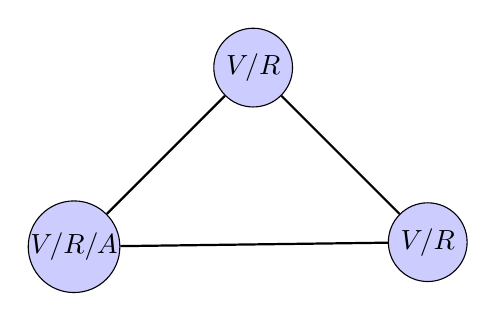
\begin{tikzpicture}
    \node[main node] (1) {$V/R$};
    \node[main node] (2) [below left = 1.5cm and 1.5cm of 1]  {$V/R/A$};
    \node[main node] (3) [below right = 1.5cm and 1.5cm of 1] {$V/R$};
    

    \path[draw,thick]
    (1) edge node {} (2)
    (2) edge node {} (3)
    (3) edge node {} (1);
    
\end{tikzpicture}

Si la heuristica1 por ejemplo hace el analisis empezando por el nodo de abajo a la izquierda que tiene 3 colores y elige el color Verde o Rojo, vamos a suponer el verde, luego continua con el que esta a su derecha, el algoritmo determina que se debe elegir el color rojo ya que sino habria conflictos. Luego al analizar el nodo superior descubre que no es posible elegir un color ya que los dos generan un conflicto, para efectos de este ejemplo vamos a suponer que elige el verde. El grafo que nos queda es el siguiente:

\tikzset{main node/.style={circle,fill=blue!20,draw,minimum size=1cm,inner sep=0pt},
            }

  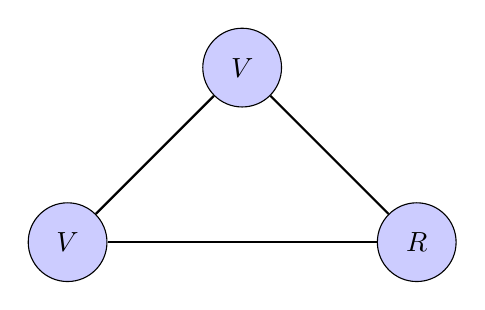
\begin{tikzpicture}
    \node[main node] (1) {$V$};
    \node[main node] (2) [below left = 1.5cm and 1.5cm of 1]  {$V$};
    \node[main node] (3) [below right = 1.5cm and 1.5cm of 1] {$R$};
    

    \path[draw,thick]
    (1) edge node {} (2)
    (2) edge node {} (3)
    (3) edge node {} (1);
    
\end{tikzpicture}

Este grafo tiene un conflito que es resoluble con la busqueda local, ya que al analizar el primer nodo es posible elegir un nuevo color, el Amarillo, lo cual al cambiarlo nos mejoraria nuestro coloreo quedando el siguiente coloreo optimo.

  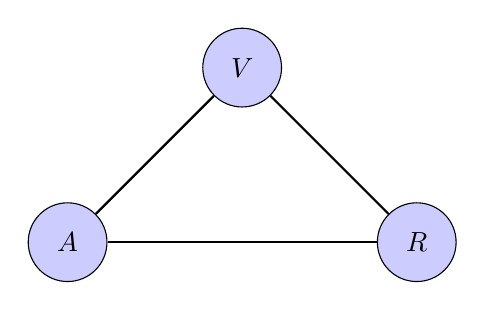
\begin{tikzpicture}
    \node[main node] (1) {$V$};
    \node[main node] (2) [below left = 1.5cm and 1.5cm of 1]  {$A$};
    \node[main node] (3) [below right = 1.5cm and 1.5cm of 1] {$R$};
    

    \path[draw,thick]
    (1) edge node {} (2)
    (2) edge node {} (3)
    (3) edge node {} (1);
    
\end{tikzpicture}